\documentclass[11pt]{article}
\usepackage[margin=1in]{geometry}
\usepackage{amsmath}
\usepackage{amssymb}
\usepackage{booktabs}
\usepackage{graphicx}
\usepackage{longtable}
\usepackage[table]{xcolor}
\usepackage[colorlinks=true,urlcolor=blue,linkcolor=black]{hyperref}
\setlength{\parskip}{0.5em}
\setlength{\parindent}{0pt}
% \texttt{ring\_count} and friends are unbreakable and otherwise poke into the
% margin; let TeX stretch interword space instead.
\sloppy


\begin{document}

\title{MDLM few-step generation: \texttt{marginal} vs \texttt{edlm} at $k$ tokens per step}

\author{QED / fewstep}

\date{2026-08-26}

\maketitle



\begin{center}
\fcolorbox{black}{yellow!25}{\begin{minipage}{0.93\textwidth}
\textbf{\large Read this before quoting any hits number in this report.}

\medskip
Every hits@0.6 figure below is counted on \texttt{novel}, defined as
$\mathrm{set(valid)} \setminus \mathrm{QM9}$, and that metric is
\textbf{confounded by molecule size in a way that scales with $k$}. QM9 contains
only molecules of $\le 9$ heavy atoms; RDKit validity does not enforce that, and
QED rewards size (it peaks near 300\,Da, far above anything QM9 can reach). Two
biases therefore compound and both grow with $k$: molecules outside the size
range are novel \emph{by construction}, and they score higher QED. Measured on
$N=1000$, $\lambda=200$, \texttt{edlm}: mean heavy-atom count runs $9.0 \to 13.6$
and the fraction above 9 heavy atoms runs $38.9\,\% \to 95.7\,\%$ as
$k: 1 \to 32$.

\medskip
Recounted on metrics that are not size-confounded (5-seed means, same runs):

\begin{center}\small
\begin{tabular}{lrrrr}
\toprule
$k$ (at $N=1000$, $\lambda=200$) & 1 & 4 & 8 & 32 \\
\midrule
as reported below (novel) & 69.6 & 111.2 & \textbf{137.4} & 98.2 \\
unique valid, no QM9 subtraction & \textbf{166.0} & 123.8 & 139.6 & 98.2 \\
restricted to $\le 9$ heavy atoms & \textbf{115.0} & 30.2 & 11.6 & 0.2 \\
\bottomrule
\end{tabular}
\end{center}

\medskip
\textbf{Invalidated:} every claim that few-step raises hits, the reward-call
Pareto frontier, and the reading of $\mathrm{novel}/\mathrm{valid}\to 1$ as
``duplication disappears'' (it is the size drift). \textbf{Still valid:} the
\texttt{marginal} vs \texttt{edlm} contrast (both modes drift identically, to
one decimal place in heavy-atom count, so it cancels in $\Delta$), the two null
controls, the validity collapse being a property of few-step itself, and the
\texttt{allbad} analysis.

\medskip
Synthetic accessibility is \emph{flat} across $k$ (SA 4.74 / 4.74 / 4.75 at
$k=1/8/32$ against 3.61 for QM9), so the larger molecules are not unmakeable
junk --- this is a confounded comparison, not reward hacking.

\medskip
Recount data: \texttt{results/qed/fewstep/\_recount.csv} (1240 runs), produced by
\texttt{scripts/ours/recount\_size\_controlled.py}. The choice of replacement
metric is an open decision; this report has not been rewritten under it.
\end{minipage}}
\end{center}

\bigskip

\section{What this sweep is}

At $k=1$ unmasked position per step the two mixture samplers are the
\emph{same Markov chain}: \texttt{marginal} returns
$\mathbb{E}_n[q(\cdot\,|\,x_t,x_0^{(n)})]$ while \texttt{edlm} draws
$n^\ast\sim\mathrm{Cat}(w)$ and samples that component, and with one position
updating the joint equals that position's marginal. The whole difference
therefore lives in steps with $k\ge 2$, where \texttt{marginal} draws each
position independently from the reward-weighted candidate histogram while
\texttt{edlm} copies $k$ tokens from a single candidate. This sweep puts $k$ on
an axis.

No code change was needed. \texttt{position\_selection=random\_k} unmasks
$\mathrm{round}(n_{\text{masked}}\cdot p_{\text{unmask}})$ positions and for the
log-linear schedule $p_{\text{unmask}} = \mathrm{d}t/t$ exactly, so
$k = L/T$ deterministically at every step; verified numerically for
$T\in\{32,16,8,4\}$ with no rounding drift and no leftover mask. Uniformly random
positions are not a heuristic here: every masked position carries the same
``stay masked'' probability, so conditional on the count the position set is
uniform over subsets --- \texttt{random\_k} \emph{is} the true kernel
conditioned on the count.

Arm A settings throughout (\texttt{oversample=1}, \texttt{exclude\_invalid=False},
\texttt{exact\_uniform\_step=False}), $N\in\{10,30,100,300,1000\}$,
$\lambda\in\{0,20,200,1000\}$, seeds $1$--$5$, 2048 samples per run.
800 runs, no failures. \textbf{Exploratory: read the trend, not a single cell.}

\section{Two built-in null controls}

Both must come out at zero. $k=1$ is the structural null above.
$\lambda=0$ is a second, independent null at \emph{every} $k$: the weights are
uniform, and the candidates were drawn position-independently from
$x_\theta$, so copying $k$ tokens from one candidate \emph{is} $k$ independent
draws from $x_\theta$. The $\lambda=0$ column below is clean everywhere
($|\Delta|\le 2.6$ at every $N$ and $k$), which is what licenses reading the
$\lambda>0$ columns as a reward-driven effect.

Tested formally rather than by eye, the $k=1$ row passes: of the 15 cells
at $\lambda>0$, exactly one exceeds $p<0.05$ against 0.8 expected by chance, and
the 15 cells at $k\ge2,\ \lambda=0$ give zero. The $\pm3$ to $\pm5$ values that
look large at $N\ge300$ are not: hit counts there are 55--82, so counting noise
makes the per-seed $\Delta$ swing by $\pm15$, and those cells have $|t|<2$.

The one cell that did exceed it --- $N=100$, $\lambda=1000$, $\Delta=-10.6$ with
all five seeds negative and $t=-7.77$ --- was rerun with ten fresh seeds and did
not replicate: seeds 6--15 give $\Delta=-3.0\pm2.8$ ($t=-1.06$) at
$\lambda=1000$ and $-0.9\pm2.3$ ($t=-0.39$) at $\lambda=200$. Its two
``impossible'' features both dissolved --- the standard deviation went
$3.05\to8.24$ (counting noise predicts 8.9) and the seed-wise correlation
between the modes went $+0.97\to+0.06$. Both were five-sample artifacts. The
out-of-sample seeds are the honest test here, since the cell was selected for
looking extreme; quoting the 15-seed pooled figure would re-import that
selection. \textbf{Verdict: noise. Both null controls hold.}

\begin{table}[htbp]
\centering
\footnotesize
\setlength{\tabcolsep}{4pt}
\resizebox{\ifdim\width>\linewidth\linewidth\else\width\fi}{!}{%
\begin{tabular}{rrrrrrr}
\toprule
$N$ & $k$ & $T$ & $\lambda=0$ & $\lambda=20$ & $\lambda=200$ & $\lambda=1000$ \\
\midrule
10 & 1 & 32 & $+1.60 \pm 1.50$ & $-0.80 \pm 3.14$ & $-1.60 \pm 3.25$ & $-1.80 \pm 3.40$ \\
 & 2 & 16 & $-1.20 \pm 2.33$ & $+1.20 \pm 3.35$ & $+1.00 \pm 3.51$ & $-1.40 \pm 3.50$ \\
 & 4 & 8 & $-2.60 \pm 2.32$ & $-3.80 \pm 1.98$ & \textbf{$-5.80 \pm 1.59$} & $-4.20 \pm 1.77$ \\
 & 8 & 4 & $+0.60 \pm 0.75$ & $+0.80 \pm 1.83$ & $+3.00 \pm 2.45$ & $+2.80 \pm 2.35$ \\
30 & 1 & 32 & $-0.60 \pm 1.66$ & $-1.80 \pm 3.31$ & $+0.60 \pm 4.95$ & $+2.00 \pm 5.50$ \\
 & 2 & 16 & $-2.60 \pm 1.44$ & $-3.80 \pm 4.69$ & $-3.80 \pm 4.45$ & $-2.00 \pm 5.97$ \\
 & 4 & 8 & $-1.40 \pm 1.21$ & $-2.80 \pm 1.24$ & $-5.60 \pm 3.96$ & $-8.00 \pm 4.68$ \\
 & 8 & 4 & $+1.20 \pm 1.36$ & $+1.40 \pm 1.44$ & $+3.80 \pm 4.03$ & $+3.20 \pm 4.32$ \\
100 & 1 & 32 & $+0.20 \pm 1.07$ & $+0.20 \pm 2.85$ & $-7.80 \pm 3.76$ & \textbf{$-10.60 \pm 1.36$} \\
 & 2 & 16 & $+0.00 \pm 1.38$ & $+1.60 \pm 2.86$ & $+4.80 \pm 2.42$ & $+6.00 \pm 3.42$ \\
 & 4 & 8 & $+0.60 \pm 1.12$ & \textbf{$-4.60 \pm 1.08$} & $-6.60 \pm 2.96$ & \textbf{$-6.40 \pm 1.57$} \\
 & 8 & 4 & $-1.00 \pm 0.77$ & $-1.60 \pm 1.94$ & $+1.80 \pm 5.02$ & $+3.20 \pm 4.41$ \\
300 & 1 & 32 & $+0.60 \pm 2.06$ & $+1.80 \pm 1.24$ & $+3.20 \pm 4.58$ & $+4.60 \pm 5.07$ \\
 & 2 & 16 & $+0.20 \pm 4.45$ & $+3.40 \pm 4.68$ & $+0.20 \pm 7.21$ & $+0.60 \pm 6.71$ \\
 & 4 & 8 & $-1.20 \pm 1.53$ & \textbf{$-7.00 \pm 2.05$} & $-9.00 \pm 7.00$ & $-4.00 \pm 10.28$ \\
 & 8 & 4 & $-0.60 \pm 0.75$ & $-9.40 \pm 4.12$ & \textbf{$-12.20 \pm 3.99$} & \textbf{$-10.80 \pm 3.81$} \\
1000 & 1 & 32 & $+1.60 \pm 2.68$ & $+4.80 \pm 2.48$ & $+2.80 \pm 6.76$ & $+1.00 \pm 3.59$ \\
 & 2 & 16 & $-1.00 \pm 2.17$ & $-3.60 \pm 3.28$ & $+2.40 \pm 3.28$ & $+0.80 \pm 3.89$ \\
 & 4 & 8 & $+1.00 \pm 2.02$ & $-5.00 \pm 3.36$ & $-9.00 \pm 4.44$ & \textbf{$-10.20 \pm 3.79$} \\
 & 8 & 4 & $-0.80 \pm 0.92$ & \textbf{$-19.00 \pm 3.27$} & \textbf{$-19.40 \pm 3.61$} & \textbf{$-17.00 \pm 3.73$} \\
\bottomrule
\end{tabular}}
\caption{$\Delta$ hits@0.6 (\texttt{marginal} $-$ \texttt{edlm}), mean $\pm$ standard error over 5 seeds. Bold marks $|\Delta| > 2.5\,\mathrm{se}$. The $\lambda=0$ column and the $k=1$ row are the two null controls. Every cell is 5 seeds; the follow-up seeds of Check~A are kept out of the grid on purpose (see text) and live in \texttt{notes/fewstep\_all\_seeds.csv}.}
\label{tab:fs-delta-hits}
\end{table}


\section{Result: \texttt{edlm} wins, and the gap grows with $k$ and $N$}

The sign is the opposite of the pre-registered prediction. Crossover was
expected to pay once parents are elites; instead the conditional-independence
error dominates. Writing $k$ positions independently breaks SMILES ring-closure
digits and brackets, which are non-separable across positions, and at $k\ge 4$
that cost swamps the extra reachable combinations. The largest effect is
$-19.4\pm3.6$ at $N=1000$, $k=8$, $\lambda=200$.

\begin{figure}[htbp]\centering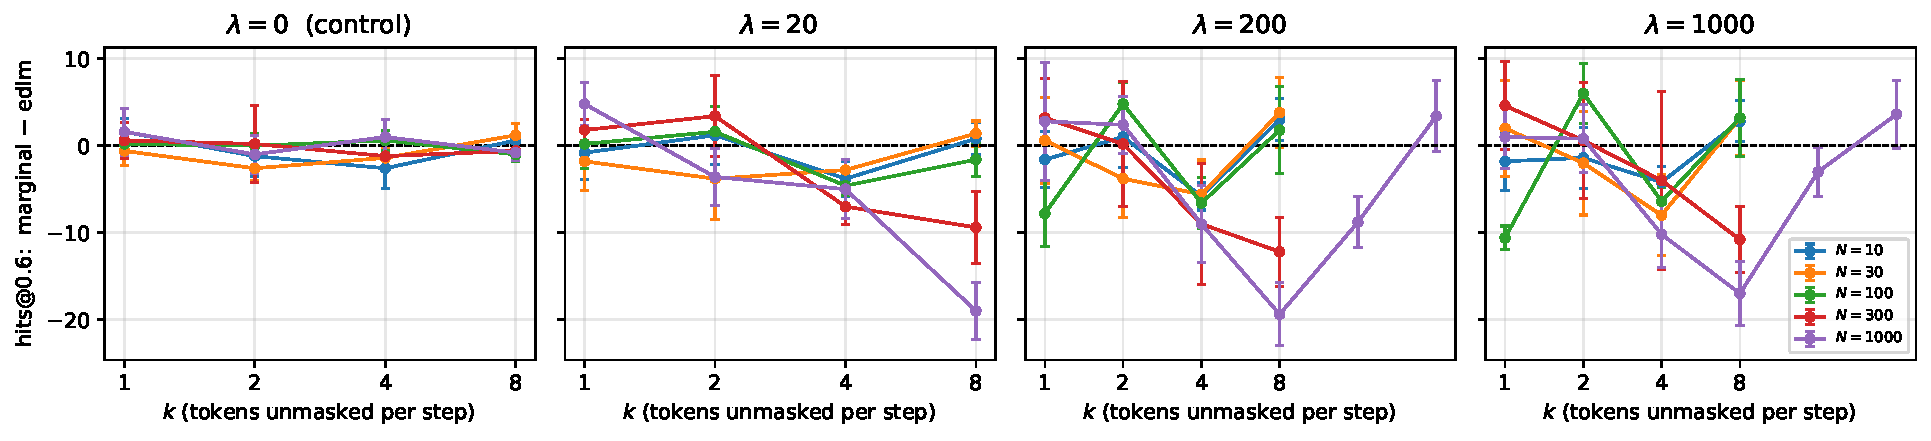
\includegraphics[width=\linewidth]{fewstep_delta.pdf}\caption{$\Delta$ hits@0.6 against $k$. $\lambda=0$ is the control panel; error bars are $\pm1$ standard error over 5 seeds.}\label{fig:fs-delta}\end{figure}

\section{The trade-off few-step actually makes}

Validity collapses with $k$ exactly as expected --- and hits go
\emph{up} anyway, \emph{for both samplers}, provided $N$ is large enough. The
best $k$ is interior and it moves right with $N$: reading Table~\ref{tab:fs-tradeoff}
by row, hits@0.6 peak at $k=2$ for $N=10$ and $N=30$, at $k=2$--$4$ for $N=100$,
at $k=4$ for $N=300$, and at $k=8$ for $N=1000$ --- where the follow-up rows
confirm it turns over, 137.4 at $k=8$ against 109.2 at $k=16$ and 98.2 at
$k=32$. Larger $N$ buys more candidates and so survives a bigger per-step commit
before the state degenerates: \texttt{allbad} at $k=8$ is 0.824 at $N=300$
against 0.728 at $N=1000$. Writing
$\mathrm{hits@0.6} = \mathrm{valid} \times
\frac{\mathrm{novel}}{\mathrm{valid}} \times
\frac{\mathrm{hits@0.6}}{\mathrm{novel}}$
splits that into three factors, and going $k=1 \to 8$ at $N=1000$ moves each one
in a different direction:

\begin{center}\small
\begin{tabular}{lcccc}
\toprule
 & valid & novel/valid & hits@0.6/novel & $=$ hits@0.6 \\
\midrule
\texttt{marginal} & $\times 0.32$ & $\times 2.09$ & $\times 2.47$ & $\times 1.63$ \\
\texttt{edlm}     & $\times 0.33$ & $\times 2.14$ & $\times 2.78$ & $\times 1.97$ \\
\bottomrule
\end{tabular}
\end{center}

Validity falls threefold, and \emph{both} of the other factors more than double,
at one eighth of the reward calls. The middle factor is the one that is easy to
miss: at $k=1$ only 45\,\% of valid molecules are novel, at $k=8$ it is 95\,\% ---
few-step buys diversity because there is far less duplication among the
survivors. The two samplers differ only in the last factor, which is exactly the
coherence effect \texttt{edlm} wins on.

\begin{table}[htbp]
\centering
\footnotesize
\setlength{\tabcolsep}{4pt}
\resizebox{\ifdim\width>\linewidth\linewidth\else\width\fi}{!}{%
\begin{tabular}{rrrr|rrrr|rrrr}
\toprule
$N$ & $k$ & $T$ & calls & valid & $\frac{\text{novel}}{\text{valid}}$ & $\frac{\text{hits@0.6}}{\text{novel}}$ & hits@0.6 & valid & $\frac{\text{novel}}{\text{valid}}$ & $\frac{\text{hits@0.6}}{\text{novel}}$ & hits@0.6 \\
\midrule
10 & 1 & 32 & 320 & 1561 & 0.33 & 0.036 & 18.4 & 1564 & 0.32 & 0.040 & 20.0 \\
 & 2 & 16 & 160 & 1106 & 0.47 & 0.045 & 23.6 & 1114 & 0.45 & 0.045 & 22.6 \\
 & 4 & 8 & 80 & 539 & 0.64 & 0.046 & 16.0 & 548 & 0.64 & 0.062 & 21.8 \\
 & 8 & 4 & 40 & 147 & 0.83 & 0.062 & 7.6 & 155 & 0.85 & 0.035 & 4.6 \\
30 & 1 & 32 & 960 & 1592 & 0.34 & 0.056 & 30.0 & 1579 & 0.34 & 0.055 & 29.4 \\
 & 2 & 16 & 480 & 1153 & 0.48 & 0.053 & 29.6 & 1145 & 0.48 & 0.060 & 33.4 \\
 & 4 & 8 & 240 & 607 & 0.68 & 0.060 & 24.4 & 623 & 0.68 & 0.071 & 30.0 \\
 & 8 & 4 & 120 & 208 & 0.89 & 0.088 & 16.4 & 202 & 0.89 & 0.070 & 12.6 \\
100 & 1 & 32 & 3200 & 1623 & 0.38 & 0.053 & 33.2 & 1611 & 0.37 & 0.069 & 41.0 \\
 & 2 & 16 & 1600 & 1206 & 0.53 & 0.081 & 52.0 & 1206 & 0.51 & 0.076 & 47.2 \\
 & 4 & 8 & 800 & 676 & 0.72 & 0.095 & 45.8 & 690 & 0.71 & 0.106 & 52.4 \\
 & 8 & 4 & 400 & 278 & 0.91 & 0.125 & 31.6 & 281 & 0.92 & 0.115 & 29.8 \\
300 & 1 & 32 & 9600 & 1647 & 0.42 & 0.084 & 58.4 & 1638 & 0.42 & 0.080 & 55.2 \\
 & 2 & 16 & 4800 & 1249 & 0.56 & 0.095 & 66.6 & 1267 & 0.55 & 0.095 & 66.4 \\
 & 4 & 8 & 2400 & 765 & 0.75 & 0.118 & 67.8 & 785 & 0.75 & 0.130 & 76.8 \\
 & 8 & 4 & 1200 & 365 & 0.93 & 0.154 & 52.2 & 381 & 0.94 & 0.180 & 64.4 \\
1000 & 1 & 32 & 32000 & 1668 & 0.45 & 0.096 & 72.4 & 1666 & 0.44 & 0.094 & 69.6 \\
 & 2 & 16 & 16000 & 1330 & 0.58 & 0.119 & 92.6 & 1341 & 0.59 & 0.115 & 90.2 \\
 & 4 & 8 & 8000 & 867 & 0.76 & 0.155 & 102.2 & 903 & 0.77 & 0.160 & 111.2 \\
 & 8 & 4 & 4000 & 527 & 0.94 & 0.237 & 118.0 & 553 & 0.95 & 0.262 & 137.4 \\
 & 16 & 2 & 2000 & 261 & 1.00 & 0.386 & 100.4 & 274 & 0.99 & 0.401 & 109.2 \\
 & 32 & 1 & 1000 & 244 & 1.00 & 0.416 & 101.6 & 243 & 1.00 & 0.405 & 98.2 \\
\bottomrule
\end{tabular}}
\caption{$\lambda=200$, counts out of 2048 samples; columns 5--8 are \texttt{marginal} and 9--12 are \texttt{edlm}. \emph{hits@0.6} is the number of \emph{novel} molecules scoring $\mathrm{QED}\ge0.60$, the same quantity as in Table~\ref{tab:fs-delta-hits}; \emph{valid} and \emph{novel} are counts of the 2048 generated sequences, and \emph{novel} is deduplicated ($\mathrm{set(valid)}\setminus$ train). Reward evaluations per sequence are $N\times T$. The three factors multiply to hits@0.6, so each row shows where few-step gains and where it pays. The $k=16$ and $k=32$ rows exist only at $N=1000$: they were a follow-up once the factorial grid put that optimum on its boundary.}
\label{tab:fs-tradeoff}
\end{table}


\section{Pushing $k$ further at $N=1000$}

Since the factorial grid put the $N=1000$ optimum on its boundary,
$k=16$ ($T=2$) and $k=32$ ($T=1$) were run there as a follow-up.
\textbf{$k=8$ really is the peak}: hits@0.6 falls from 137.4 to 109.2 to 98.2.
But the reward budget halves each time, so hits \emph{per call} keeps rising ---
34.4, 54.6 and 98.2 per 1000 calls --- and $k=32$ stays on the frontier.

Two things fall out. First, the mode difference \textbf{vanishes again} at
$k=32$ ($\Delta=+3.4$, $t=0.84$), and the effective sample size says why. Steps
where no candidate parses carry uniform weights and hence $\mathrm{ESS}=N$
exactly, so removing them recovers the concentration in the steps that matter:
$\mathrm{ESS}_{\text{live}} = (\mathrm{ESS} - \texttt{allbad}\cdot N)/(1-\texttt{allbad})$
falls $302 \to 61 \to 1.5$ for $k = 1 \to 8 \to 32$. At 1.5 effective parents the
weighted histogram is a one-hot, so \texttt{marginal} \emph{is} \texttt{edlm}.
The difference peaks at $k=8$ because that is where the concentration is
intermediate --- the same non-monotonicity predicted for $\lambda$, arriving
through $k$ instead.

Second, $T=1$ gives a free implementation check. With one step \texttt{edlm}
returns a candidate verbatim (it is literally best-of-$N$), so if the reward ever
picks a parseable candidate the output must be valid, i.e.
$\mathrm{valid} = 1 - \texttt{allbad}$. Measured: $\texttt{allbad}=0.874$
predicts 0.126 against 0.118 observed.

\begin{table}[htbp]
\centering
\small
\resizebox{\ifdim\width>\linewidth\linewidth\else\width\fi}{!}{%
\begin{tabular}{rrrrrrrr}
\toprule
$k$ & $T$ & reward calls & \texttt{marginal} & \texttt{edlm} & $\Delta$ & $t$ & hits per 1000 calls \\
\midrule
1 & 32 & 32000 & 72.4 & 69.6 & $+2.8$ & $+0.41$ & 2.3 \\
2 & 16 & 16000 & 92.6 & 90.2 & $+2.4$ & $+0.73$ & 5.8 \\
4 & 8 & 8000 & 102.2 & 111.2 & $-9.0$ & $-2.03$ & 13.9 \\
8 & 4 & 4000 & 118.0 & 137.4 & $-19.4$ & $-5.37$ & 34.4 \\
16 & 2 & 2000 & 100.4 & 109.2 & $-8.8$ & $-3.01$ & 54.6 \\
32 & 1 & 1000 & 101.6 & 98.2 & $+3.4$ & $+0.84$ & 101.6 \\
\bottomrule
\end{tabular}}
\caption{$N=1000$, $\lambda=200$, hits@0.6. $k=16$ and $32$ are a follow-up at this $N$ only. Absolute hits peak at $k=8$; hits per reward call keep rising to $k=32$.}
\label{tab:fs-extension}
\end{table}


\section{Hits per reward call: no $k=1$ point is on the frontier}

This is the axis the reframed claim needs (hits against reward-call
budget). Every point on the Pareto front has $k\ge 2$. The previous operating
point ($N=300$, $k=1$, $T=32$, $\lambda=200$: 55.2 hits at 9600 calls) is well
inside it --- $N=300$, $k=4$ gives 78.4 hits at 2400 calls, i.e.
$4\times$ fewer reward evaluations and 42\,\% more hits.

\begin{table}[htbp]
\centering
\small
\resizebox{\ifdim\width>\linewidth\linewidth\else\width\fi}{!}{%
\begin{tabular}{rrrrrrl}
\toprule
reward calls & hits@0.6 & $N$ & $k$ & $T$ & $\lambda$ & mode \\
\midrule
40 & 7.6 & 10 & 8 & 4 & 200 & marginal \\
40 & 7.6 & 10 & 8 & 4 & 1000 & marginal \\
80 & 21.8 & 10 & 4 & 8 & 200 & edlm \\
160 & 24.4 & 10 & 2 & 16 & 1000 & edlm \\
240 & 33.0 & 30 & 4 & 8 & 1000 & edlm \\
400 & 33.6 & 100 & 8 & 4 & 1000 & marginal \\
480 & 34.6 & 30 & 2 & 16 & 1000 & edlm \\
800 & 54.0 & 100 & 4 & 8 & 1000 & edlm \\
1000 & 101.8 & 1000 & 32 & 1 & 1000 & marginal \\
2000 & 110.4 & 1000 & 16 & 2 & 1000 & edlm \\
4000 & 142.0 & 1000 & 8 & 4 & 1000 & edlm \\
\bottomrule
\end{tabular}}
\caption{Pareto frontier of hits@0.6 against reward evaluations per sequence ($\lambda>0$ only).}
\label{tab:fs-frontier}
\end{table}


\begin{figure}[htbp]\centering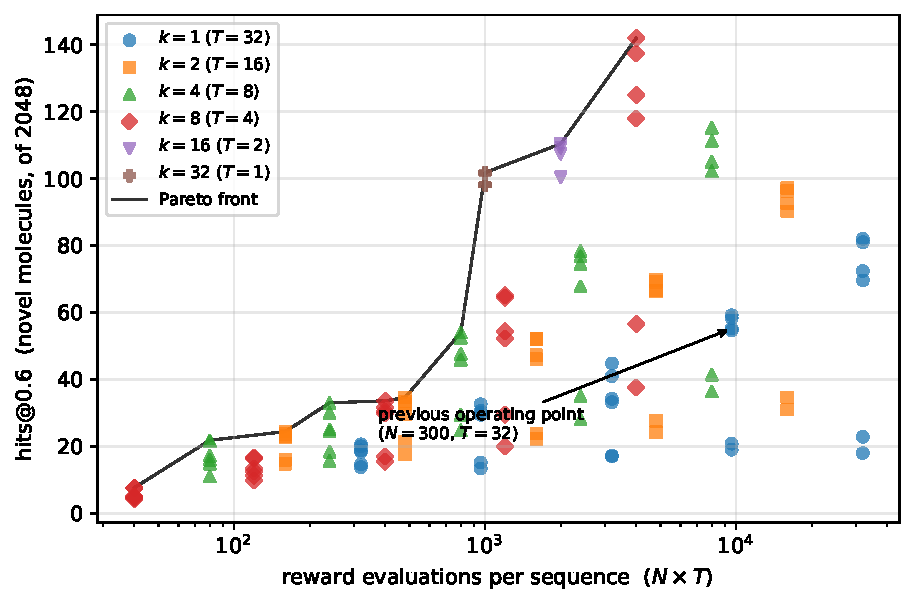
\includegraphics[width=0.78\linewidth]{fewstep_frontier.pdf}\caption{Every cell of the sweep, hits against reward budget.}\label{fig:fs-frontier}\end{figure}

\section{Validity, as a difference}

\begin{table}[htbp]
\centering
\footnotesize
\setlength{\tabcolsep}{4pt}
\resizebox{\ifdim\width>\linewidth\linewidth\else\width\fi}{!}{%
\begin{tabular}{rrrrrrr}
\toprule
$N$ & $k$ & $T$ & $\lambda=0$ & $\lambda=20$ & $\lambda=200$ & $\lambda=1000$ \\
\midrule
10 & 1 & 32 & $-7.8 \pm 14.57$ & $-0.6 \pm 13.43$ & $-3.2 \pm 14.65$ & $-0.8 \pm 13.92$ \\
 & 2 & 16 & $-12.4 \pm 13.19$ & $-9.4 \pm 8.45$ & $-7.8 \pm 6.82$ & $-5.8 \pm 7.37$ \\
 & 4 & 8 & $-6.0 \pm 8.07$ & $-10.2 \pm 11.52$ & $-9.4 \pm 12.98$ & $-8.4 \pm 13.49$ \\
 & 8 & 4 & \textbf{$-3.4 \pm 1.03$} & $-12.2 \pm 8.57$ & $-7.8 \pm 7.66$ & $-7.8 \pm 7.56$ \\
30 & 1 & 32 & $+20.2 \pm 11.59$ & $+10.4 \pm 6.07$ & \textbf{$+13.6 \pm 3.49$} & \textbf{$+11.2 \pm 4.19$} \\
 & 2 & 16 & $-2.2 \pm 12.29$ & $+1.4 \pm 7.85$ & $+7.6 \pm 12.10$ & $+10.2 \pm 11.06$ \\
 & 4 & 8 & $-1.8 \pm 10.65$ & $-20.6 \pm 15.59$ & $-15.8 \pm 13.48$ & $-13.2 \pm 12.46$ \\
 & 8 & 4 & $+3.8 \pm 5.59$ & $+1.2 \pm 9.12$ & $+6.6 \pm 10.52$ & $+7.4 \pm 10.60$ \\
100 & 1 & 32 & $+1.8 \pm 14.84$ & $+15.0 \pm 14.96$ & $+12.6 \pm 9.04$ & $+10.4 \pm 8.82$ \\
 & 2 & 16 & $-10.4 \pm 15.38$ & $-12.0 \pm 20.39$ & $+0.2 \pm 19.27$ & $+0.6 \pm 18.66$ \\
 & 4 & 8 & $-1.6 \pm 14.15$ & \textbf{$-31.4 \pm 8.02$} & $-14.4 \pm 9.81$ & $-8.6 \pm 9.06$ \\
 & 8 & 4 & $+2.6 \pm 3.71$ & $-18.6 \pm 9.19$ & $-3.2 \pm 8.30$ & $+4.6 \pm 8.57$ \\
300 & 1 & 32 & $+8.4 \pm 11.11$ & $+1.8 \pm 12.01$ & $+8.6 \pm 11.23$ & $+7.0 \pm 13.07$ \\
 & 2 & 16 & $-3.2 \pm 11.43$ & $-23.6 \pm 21.44$ & $-18.2 \pm 19.51$ & $-12.6 \pm 19.21$ \\
 & 4 & 8 & $+11.6 \pm 11.40$ & \textbf{$-43.0 \pm 6.88$} & \textbf{$-20.0 \pm 7.98$} & $-13.6 \pm 9.31$ \\
 & 8 & 4 & $+9.6 \pm 7.08$ & \textbf{$-56.2 \pm 5.29$} & $-15.6 \pm 8.47$ & $-9.0 \pm 9.08$ \\
1000 & 1 & 32 & $+5.0 \pm 14.65$ & $+7.6 \pm 7.85$ & $+1.4 \pm 8.52$ & $+6.2 \pm 9.77$ \\
 & 2 & 16 & $+11.8 \pm 9.74$ & $-16.4 \pm 11.09$ & $-11.0 \pm 13.97$ & $-13.8 \pm 11.20$ \\
 & 4 & 8 & $+3.0 \pm 7.84$ & \textbf{$-76.6 \pm 10.84$} & \textbf{$-35.4 \pm 5.38$} & \textbf{$-35.2 \pm 9.10$} \\
 & 8 & 4 & $-7.2 \pm 2.92$ & \textbf{$-105.4 \pm 7.26$} & \textbf{$-26.0 \pm 6.64$} & $-11.6 \pm 9.81$ \\
\bottomrule
\end{tabular}}
\caption{$\Delta$ valid molecules out of 2048 (\texttt{marginal} $-$ \texttt{edlm}), 5 seeds; bold marks $|\Delta| > 2.5\,\mathrm{se}$. The validity cost of per-position mixing is confirmed only at $\lambda=20$, $k\ge4$, large $N$ (and $\lambda=200$, $N=1000$, $k=8$). Cells where \texttt{marginal} comes out ahead reach at most $t=+1.4$, i.e. none of them is distinguishable from zero --- the mixed signs elsewhere are noise on a standard error of 5--20 counts.}
\label{tab:fs-delta-valid}
\end{table}


\section{Predictions, scored}

\begin{table}[htbp]
\centering
\small
\resizebox{\ifdim\width>\linewidth\linewidth\else\width\fi}{!}{%
\begin{tabular}{ll}
\toprule
prediction & outcome \\
\midrule
$k=1 \Rightarrow \Delta=0$ & partly --- 2 of 20 cells deviate \\
$\lambda=0 \Rightarrow \Delta=0$ & \textbf{held} at every $N$, $k$ \\
$N=10$, $k\ge2 \Rightarrow \Delta\approx0$ & held, small and mixed \\
$N\uparrow$, $k\uparrow \Rightarrow |\Delta|$ grows & magnitude \textbf{held}, sign \textbf{wrong} \\
$\lambda\le50 \Rightarrow \Delta<0$ & held --- but $\lambda\ge200$ is negative too \\
$k$ large $\Rightarrow \Delta$ collapses (\texttt{allbad}$\to1$) & \textbf{wrong} --- $k=8$ is the maximum \\
\bottomrule
\end{tabular}}
\caption{Written down before the sweep was read.}
\label{tab:fs-predictions}
\end{table}


\section{What is and is not resolvable here}

Seed-to-seed noise was measured directly from five existing replicates
(\texttt{random\_k}, marginal, $N=300$, 1024 samples): single-run standard
deviation 3.58 on hits@0.6, 7.3 on valid, 0.0046 on novel-QED mean, 0.010 on
max. At 2048 samples with 5 seeds this gives $\mathrm{se}\approx1.6$ on the
paired hits difference. Consequences: hits@0.6 and hits@0.65 are the only
metrics that resolve this comparison; \texttt{max} has a noise floor several
times its own effect and is reported only for honesty; the count of novel
molecules is null on the mode axis because the validity loss and the diversity
gain cancel, and is the right metric for the $k$ axis instead.

\end{document}